
% ter??
% DUE = DNA unwinding element

%% KARTEIKARTEN
% Genomtypen von viren und eukaryoten?
% Was machen SMC genau ( auch hier im Blatt!!)
% The effect of Fis on nucleoid structure and gene expression
% generelle Transduktion 
% ineare Replikation unter Bildung von Haarnadelstrukturen
% ablauf f plasmif und konjugation und so 
% was ist die nic site?
% Kartierung via transoformtaion (54)
 
 
 
 
 
 % Ausgelassen: 
 % Folie 32 und 33, 35
 % Ablauf kloniweung muss in Prak 

\section{Typen von prokaryotischen Genomen}
\begin{table}[H]
    \centering
    \begin{tabular}{p{2cm}p{4cm}p{5cm}p{5cm}}
        Genom-Typ & \textbf{Viral} & \textbf{Prokaryotisch} & \textbf{Eukaryotisch} \\
        \textbf{Struktur} & RNA / DNA in diversen Formen & zirkuläres Chromosom (meistens eines) & lineare Chromosome \\
        \textbf{Material} & RNA oder DNA & DNA & DNA 
    \end{tabular} \index{Genom!virales} \index{Genom!prokaryotisches} \index{Genom!eukaryotisches}
    \caption{Vergleich zwischen viralen, prokariotischen und eukaryotischen Genomen.}
    \label{tab:genomtypen}
\end{table}
Takeaway: Virale Genome sind deutlich anders als prokaryotische und eukaryotische Genome und können auch aus RNA bestehen!
\subsection{Prokaryotische Genome} \index{Genom!prokaryotisches}
\begin{figure}[H]
    \centering
\begin{subfigure}{0.2\textwidth}
    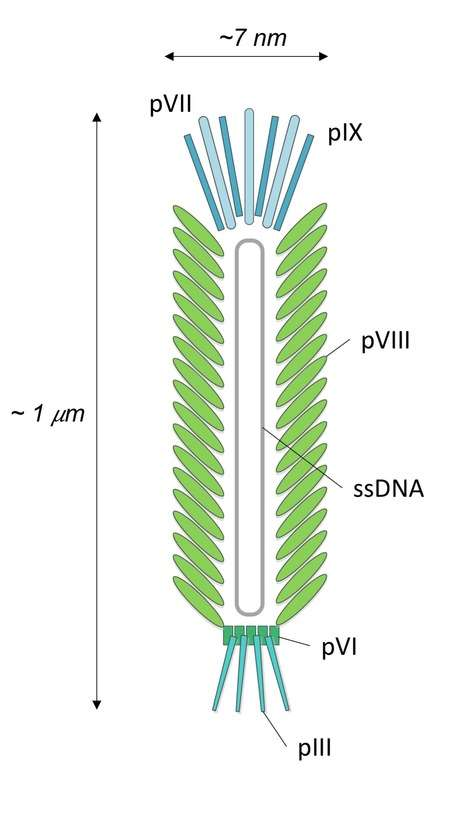
\includegraphics[height=\textwidth]{images/filamentous.jpg}
    \caption{Filamentous}
    \label{fig:filamentous}
\end{subfigure} 
\hfill
\begin{subfigure}{0.3\textwidth}
    
\includegraphics[width=\textwidth]{headtail.jpg}
    \caption{Head-and-tail}
    \label{fig:headtail}
\end{subfigure}
 \hfill  
 \begin{subfigure}{0.4\textwidth}
    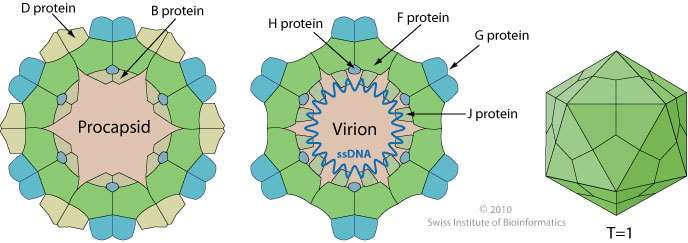
\includegraphics[width=\textwidth]{images/Icosahedral.jpg}
    \caption{Icosahedral}
    \label{fig:icosahedral}
\end{subfigure}
    \caption{Kapsid-Strukturen von Bakteriophagen.}
    \label{fig:kapsidstrukturen}
\end{figure} \index{Kapsid-Strukturen} \index{Bakteriophage}

\begin{figure}[H]
    \centering
    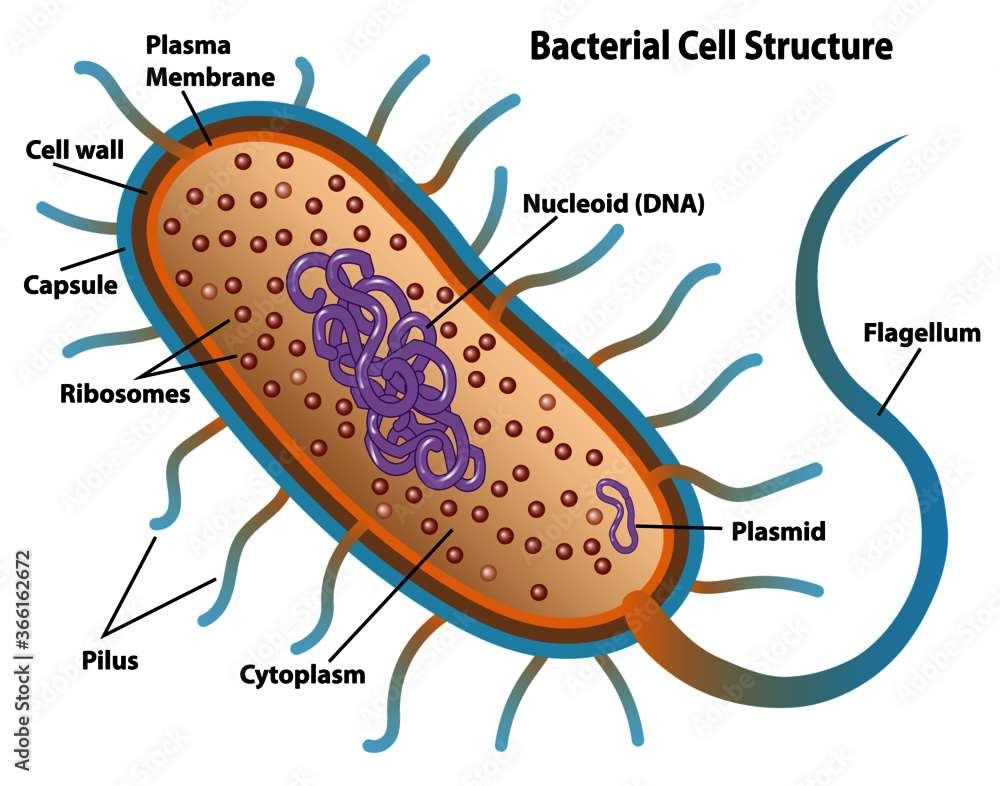
\includegraphics[width=8cm ]{images/bacterialcellstructure.jpg}
    \caption{Prokaryotische Zellen haben keinen Zellkern, sondern das Nukleoid bzw. die nukleoide Region. }
    \label{fig:nukleoid}
\end{figure}

\subsection{Virale Genome} \index{Genom!virales}
\begin{table}[H]
    \centering
    \begin{tabular}{p{5cm}p{11cm}}
        \textbf{Virus} & \textbf{Typ} \\ \hline
        Adenovirus & Doppelsträngig, linear (DNA)  \\
        Reovirus & Doppelsträngig, segmentiert, linear  (RNA)\\ \hline
        Hepatitis B & Teilweise doppelsträngig, zirkulär (DNA) \\
        SV40 & Doppelsträngig, zirkulär \\ \hline
        Influenza & Einzelsträngig, segmentiert, linear (RNA) \\ 
        Parvovirus & Einzelsträngig, linear (DNA) \\
        Polio & Einzelsträngig, linear (RNA) 
    \end{tabular}
    \caption{Beispiele von viralen Genomen.}
    \label{tab:viralgenomes}
\end{table}
\noindent Takeaway: Virale Genome sind sehr variabel und divers!
\begin{mybox}[title=Was bedeutet teilweise doppelsträngig?]
Das beschreibt DNA-Moleküle, die sowohl doppelsträngige als auch einzelsträngige Abschnitte enthalten. Siehe Hepatitis (Fig. \ref{fig:hepatitisb}). \\ Die Fähigkeit, sowohl doppelsträngige als auch einzelsträngige DNA-Abschnitte zu haben, ermöglicht es Zellen, flexibel auf verschiedene metabolische Anforderungen zu reagieren, insbesondere während der Replikation und Genexpression.
\end{mybox}
\begin{figure}[]
    \centering
\begin{subfigure}{0.4\textwidth}
    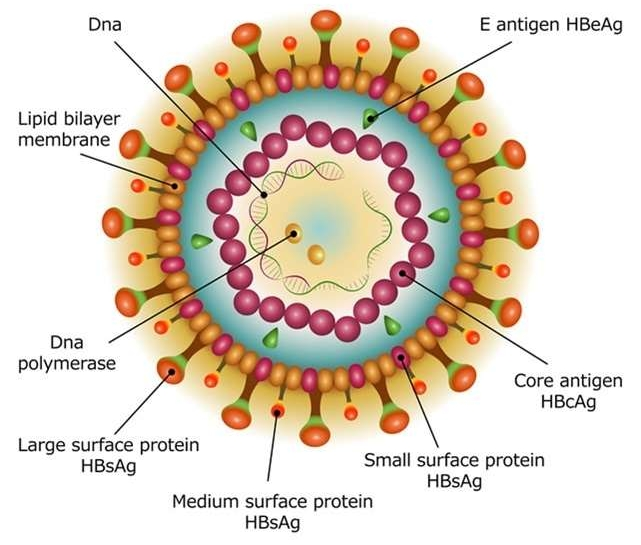
\includegraphics[width=\textwidth]{images/hepatitisb.jpg}
    \caption{Hepatitis B}
    \label{fig:hepatitisb}
\end{subfigure} 
\hfill
\begin{subfigure}{0.4\textwidth}
    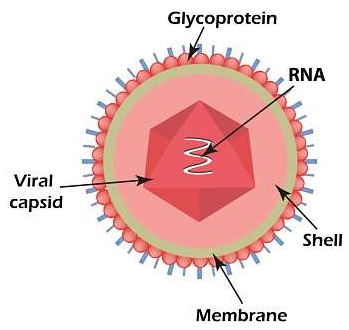
\includegraphics[width=\textwidth]{images/polio.jpg}
    \caption{Polio}
    \label{fig:polio}
\end{subfigure}
 \hfill  
 \begin{subfigure}{0.4\textwidth}
    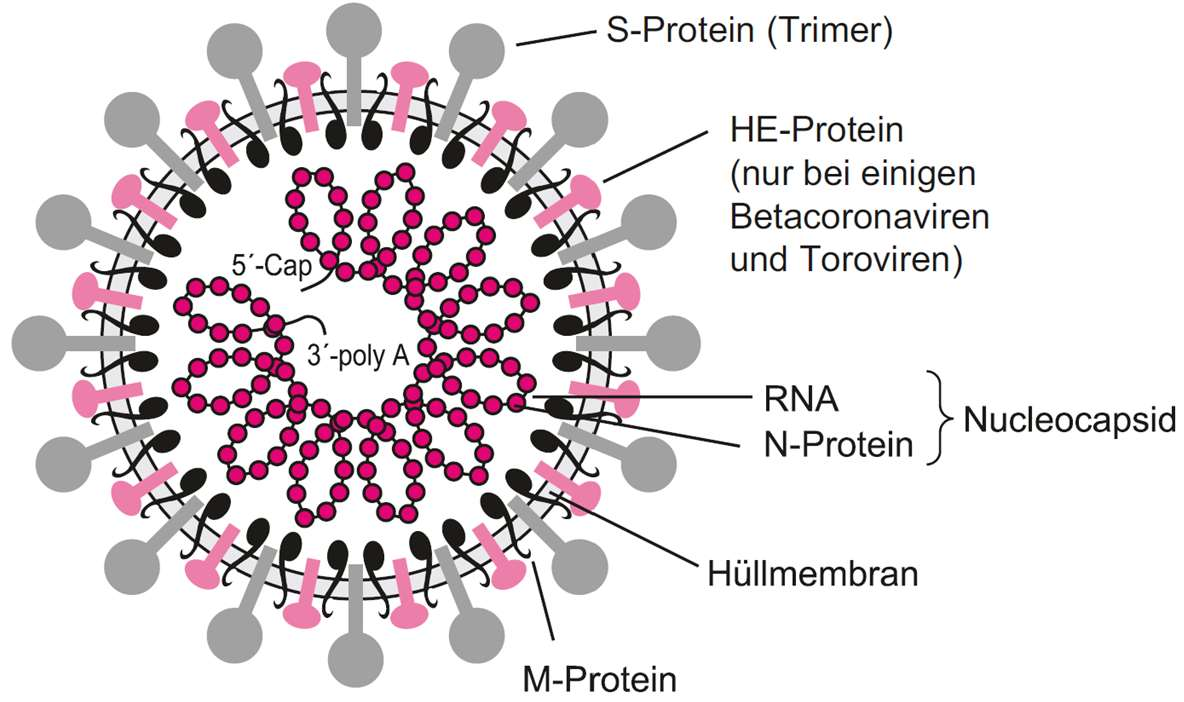
\includegraphics[width=\textwidth]{images/covid.jpg}
    \caption{Covid}
    \label{fig:covid}
\end{subfigure}
    \caption{Strukturen von ausgewählten Viren}
    \label{fig:virenstrukturen}
\end{figure}


\section{Intrinsische Eigenschaften von DNA}
\index{Topologie}
\begin{figure}[H]
    \centering
   \begin{subfigure}[t]{0.4\textwidth}
    
\includegraphics[width=\textwidth]{images/relaxeddna.jpg}
    \caption{Relaxierte DNA: der natürliche Zustand ohne topologische Spannungen (Verdrillungen).}
    \label{fig:relaxeddna}
\end{subfigure}  \index{DNA!relaxierte}
\hfill
\begin{subfigure}[t]{0.4\textwidth}
    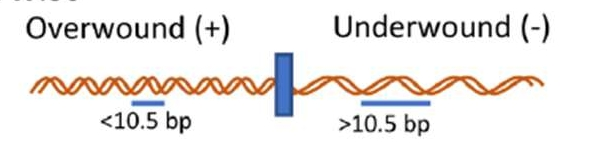
\includegraphics[width=\textwidth]{images/twidteddna.jpg}
    \caption{Verdrehte DNA: mit vollständigen Umdrehungen des Helix um die eigene Achse.}
    \label{fig:twisteddna}
\end{subfigure} \index{DNA!twisted}
\hfill
\begin{subfigure}[t]{0.4\textwidth}
    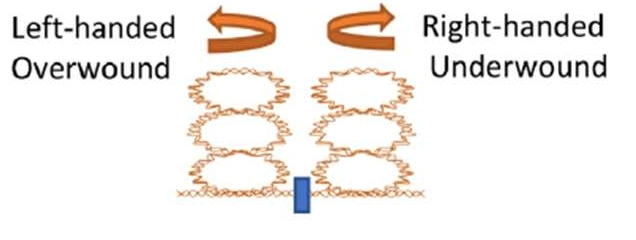
\includegraphics[width=\textwidth]{images/writheddna.jpg}
    \caption{Lokale Spiralen in der DNA durch Über- bzw. Unterwindungen und die dadurch enstehende dreidimensionale Faltung.}
    \label{fig:writheddna} 
\end{subfigure} \index{DNA!writhed}
\hfill
\begin{subfigure}[t]{0.4\textwidth}
    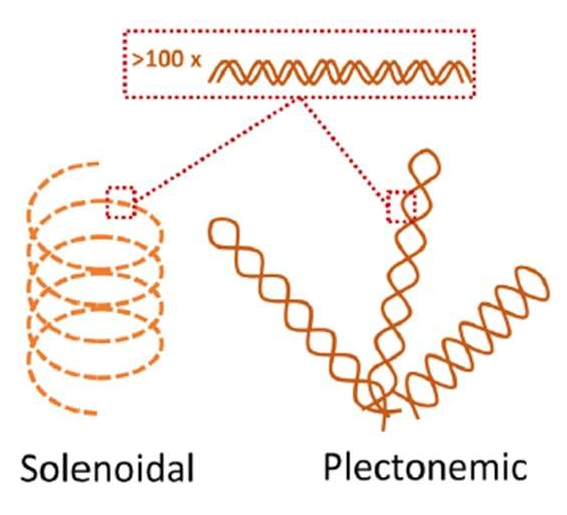
\includegraphics[width=\textwidth]{images/supercoils.jpg}
    \caption{Supercoils: Form der DNA, die entweder positiv oder negativ überdreht ist.}
    \label{fig:supercoils} 
\end{subfigure} \index{DNA!supercoiled} \index{Supercoil}
    \caption{Torsion und Überdrehung von DNA.}
    \label{fig:dnatorsionen}
\end{figure}

\begin{figure}[H]
    \centering
    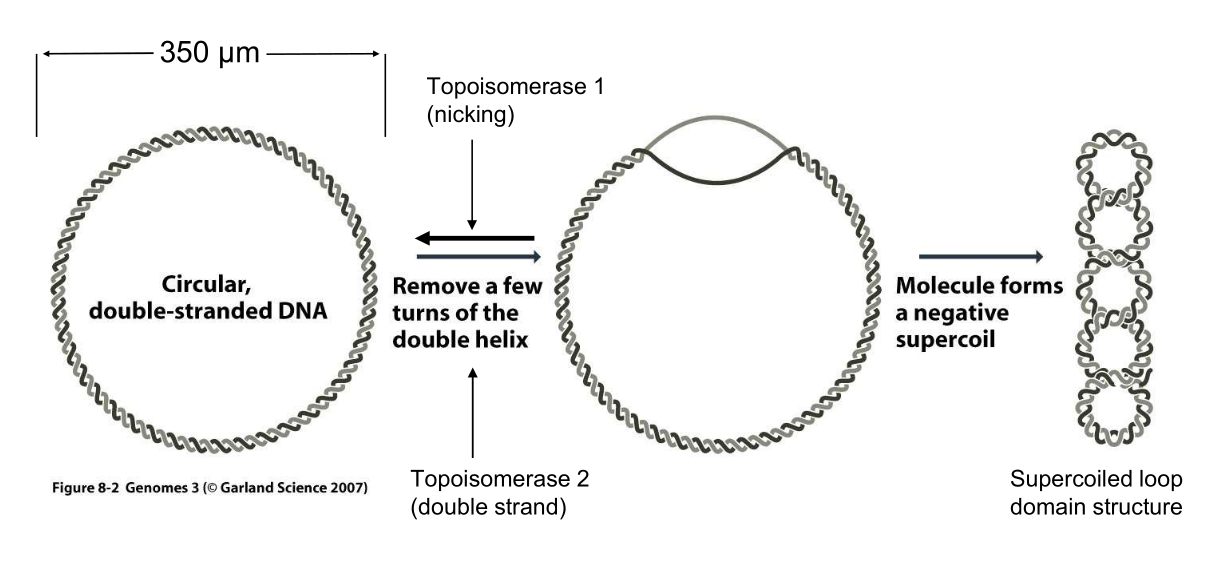
\includegraphics[width=12cm]{images/supercoiling.png}
    \caption{Prozess des Supercoiling.}
    \label{fig:supercoiling}
\end{figure} \index{Supercoil}
Supercoiled DNA \index{DNA!supercoiled} kommt in jeder lebenden Zelle vor. Sie sorgt dafür, dass stets eine Mindestmenge von Basenpaaren geöffnet ist, um so den Polymerasen zu ermöglichen, den Vorlage-Strang zum neuen Doppelstrang zu ergänzen. Dieses gilt für die Replikation und für die Transkription. Es kommt zu einem Gleichgewicht zwischen zwei so genannten Topoisomerasen.  \index{Topoisomerase}
\begin{table}[H]
    \begin{tabular}{p{4cm}p{11cm}}
        \textbf{Topoisomerase I} &  Schneidet zwei Stränge und verklebt sie. Dieser Vorgang benötigt Energie und ist daher ATP-abhängig\\
        \textbf{Topoisomerase II} & Benötigt keine Energie und entfernt das „Supercoil“, indem sie nur einen Strang schneidet, sich um den geschlossenen Strang dreht und die Lücke wieder verschließt.
    \end{tabular}
\end{table}
\begin{figure}[H]
    \centering
    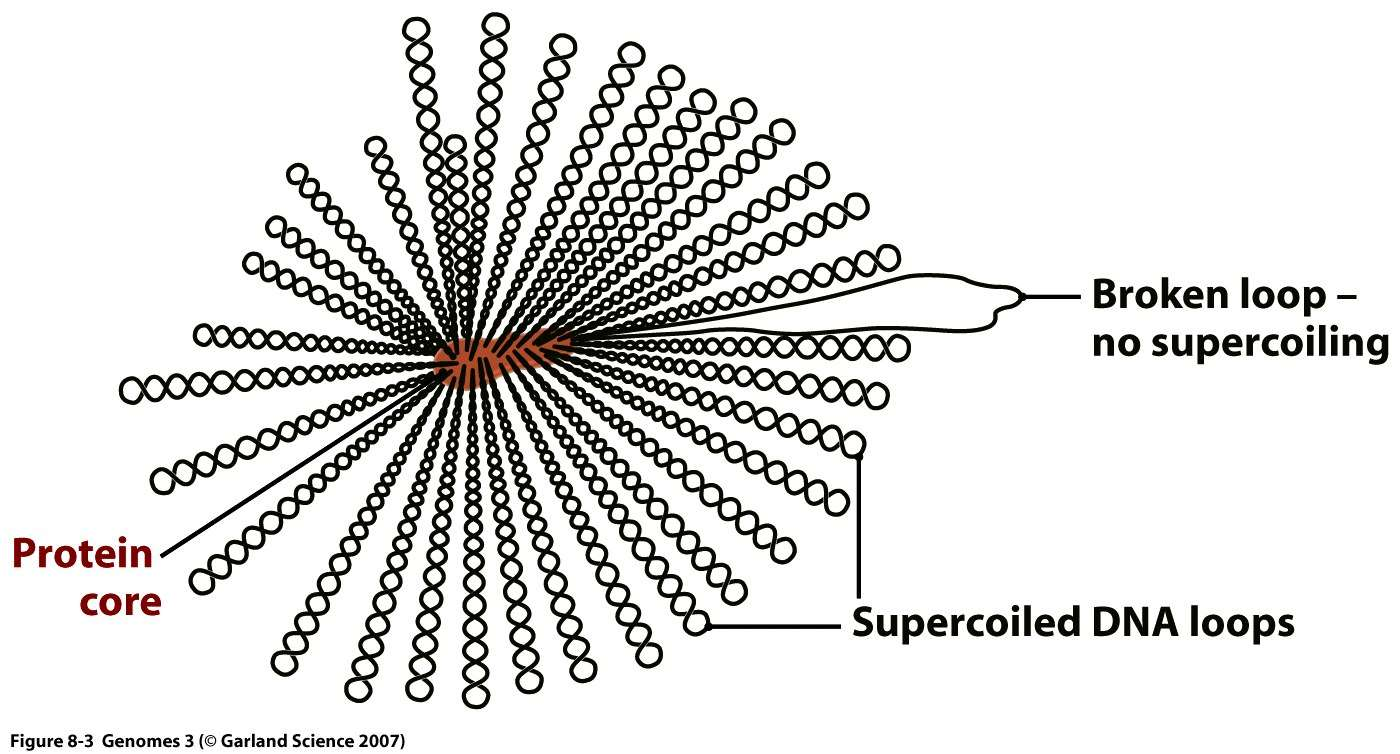
\includegraphics[width=10cm]{images/supercoiling2.jpg}
    \caption{Supercoiling des bakteriellen Chromosoms.}
    \label{fig:bacterialsupercoiling}
\end{figure} \index{Chromosom!bakterielles}

\begin{figure}[H]
    \centering
    \begin{subfigure}[t]{0.4\textwidth}
    
\includegraphics[width=\textwidth]{images/alphadna.jpg}
    \caption{Alpha-Form: Ein rechtsgängiger Helix, der einen größeren Durchmesser hat.} \index{DNA!Alpha-Form}
    \label{fig:alphadna}
\end{subfigure}
\hfill
\begin{subfigure}[t]{0.4\textwidth}
    
\includegraphics[width=\textwidth]{images/betadna.jpg}
    \caption{Beta-Form: Ein rechtsgängiger Helix, der die häufigste Form der DNA ist und sich durch einen spezifischen Abstand zwischen den Basen auszeichnet.} 
    \label{fig:betadna}
\end{subfigure} \index{DNA!Beta-Form}
    \caption{Strukturelle Formen von DNA.}
    \label{fig:dnaformen}
\end{figure}

\section{Nucleotid-associated Proteins (NAPs)} \index{Nucleotid-associated Protein}
\begin{table}[H]
    \centering
    \scriptsize
    \begin{tabular}{p{1.5cm}p{2cm}p{2cm}p{2cm}p{2cm}p{2cm}p{2cm}}
         & \normalsize \textbf{HU}  & \normalsize\textbf{H-NS} & \normalsize\textbf{Fis} & \normalsize\textbf{IHF}  &   \normalsize\textbf{Dps}   & \normalsize\textbf{MukBEF} \\  \\
        
        Funktion & bindet und stabilisiert DNA & beeinflusst DNA Topologie; Regulation der Genexpression & beeinflusst Initiation der DNA Replikation & fördert Schleifenbildung & induziert kistallinähnlichen stabilen DNA Zustand zum Schutz & Structural maintenace chromosomes (SMC)\\ \\
        Struktur & 18kDa Homo /Heterodimer & 15.5kDa Homodimer / Polymer & 11.2kDa Homodimer & 11.4 kDa Heterodimer & 18.7 kDA Ferritin-like dodecamer & 170 kDa Homodimer \\ \\
         & hupA u. hupB & H-NS & fis & ihrA u. ihfB & dps & MukB u. MukE u. MukF \\ \\
        Spezifität & keine; präferiert AT-rich & keine; präferiert AT-rich mit intrinsischer Krümmung & keine; präferiert AT-rich & 5'-WATCAANNNNTTR-3' &  \\ \\
        Konservation & min. eine Untereinheit in fast allen bakteriellen Genomen & hochgradig in E. coli und ähnlichen Stämmen & in Enterobacteriaceae & \\ \\
    \end{tabular}
    \caption{Vergleich der vercshiedenen NAPs.}
    \label{tab:napvergleich}
\end{table} \index{Nucleotid-associated Protein!H-NS} \index{Nucleotid-associated Protein!Fis} \index{Nucleotid-associated Protein!HU} \index{Nucleotid-associated Protein!MukBEF} \index{Nucleotid-associated Protein!SMC} \index{Nucleotid-associated Protein!IHF} \index{Nucleotid-associated Protein!Dps}
\index{Heterodimer} \index{Homodimer} \index{Homopolymer}

\begin{mechanism}[title=Nennen Sie 3 NAPs.]
\begin{itemize}
    \item HU
    \item H-NS
    \item Fis
\end{itemize}
\end{mechanism}

\begin{table}[H]
    \centering
    \begin{tabular}{p{3cm}p{3cm}p{3cm}p{3cm}}
        \textbf{Bridging I}  & \textbf{Bridging II} & \textbf{Stiffening} & \textbf{Bending} \\ \\
        H-NS, Fis & SMC & H-NS & Fis, HU, IHF 
    \end{tabular}
    \caption{Arten von Einfluss der NAPs auf die DNA-Struktur.}
    \label{tab:napeinfluss}
\end{table} \index{Bridging}  \index{Bending} \index{Stiffening}

\begin{mybox}[title=Was unterscheidet Histon-ähnliche Proteine von tatsächlichen Histonen? ]
 Histon-ähnliche Proteine wie HU und HNS sind Prokaryoten-spezifische Proteine, die DNA binden und stabilisieren, während echte Histone in Eukaryoten eine zentrale Rolle bei der DNA-Verpackung und -Regulation spielen.  \\ Weitere Unterschiede liegen in der Struktur, Funktion, dem Vorkommen und den Modifikationsmechanismen dieser Proteine.
\end{mybox}
\begin{mybox}[title=Homo- und Heterodimere und -polymere]
Ein Homodimer ist ein Molekül, das aus zwei identischen Untereinheiten (Monomeren) besteht, die durch nicht-kovalente Wechselwirkungen (wie Wasserstoffbrücken, ionische Bindungen oder hydrophobe Wechselwirkungen) oder kovalente Bindungen zusammengehalten werden. Ein Homopolymer ist ein Polymer, das aus mehreren identischen Monomereinheiten besteht.  \\
 Ein Heterodimer ist ein Protein, das aus zwei unterschiedlichen Untereinheiten (Monomeren) besteht. Diese Untereinheiten können aus verschiedenen Aminosäuresequenzen bestehen und unterschiedliche Eigenschaften aufweisen. \index{Heterodimer} \index{Homodimer} \index{Homopolymer}
\end{mybox} 
\subsection{Heat-unstabel protein (HU)} \index{Nucleotid-associated Protein!HU}
 \begin{itemize}
 \item Histon-ähnlich
     \item Beteiligt an Bildung der DNA Topologie und Verpackung in Nukleotid
     \item induziert negatives Supercoiling in zirkuläre DNA m.H. von Topoisomerase
     \item Hilft bei long-range Interaktionen, durch die Strukturen höherer Ordnung
     \item Bindet an veränderte DNA (Nicks, Gaps, Forks, Overhangs)
 \end{itemize}
 
\subsection{Histone-like Structuring protein (H-NS)} \index{Nucleotid-associated Protein!H-NS}
\begin{itemize}
\item Histon-ähnlich
    \item Überbrückung zwischen relativ entfernten DNA Molekülen
    \item Schränkt short-range interactions ein
    \item Xenogenic silencing
\end{itemize}
\begin{multicols}{2}
\begin{figure}[H]
    \centering
    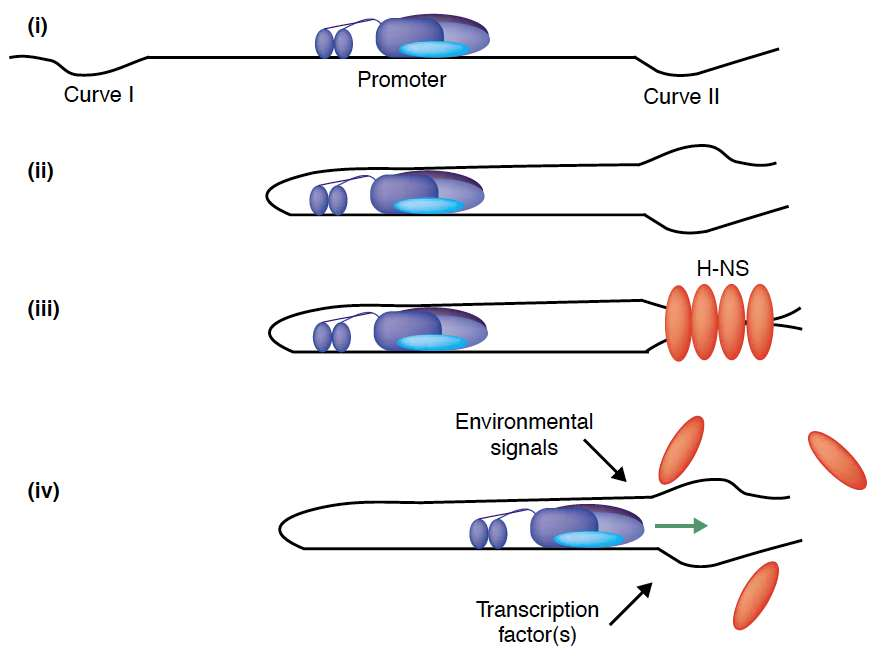
\includegraphics[width=8cm]{images/hnsrepression.jpg}
    \caption{Prozess der Repression der Transkription durch H-NS.}
    \label{fig:hnsrepression}
\end{figure}
\columnbreak
\begin{figure}[H]
    \centering
    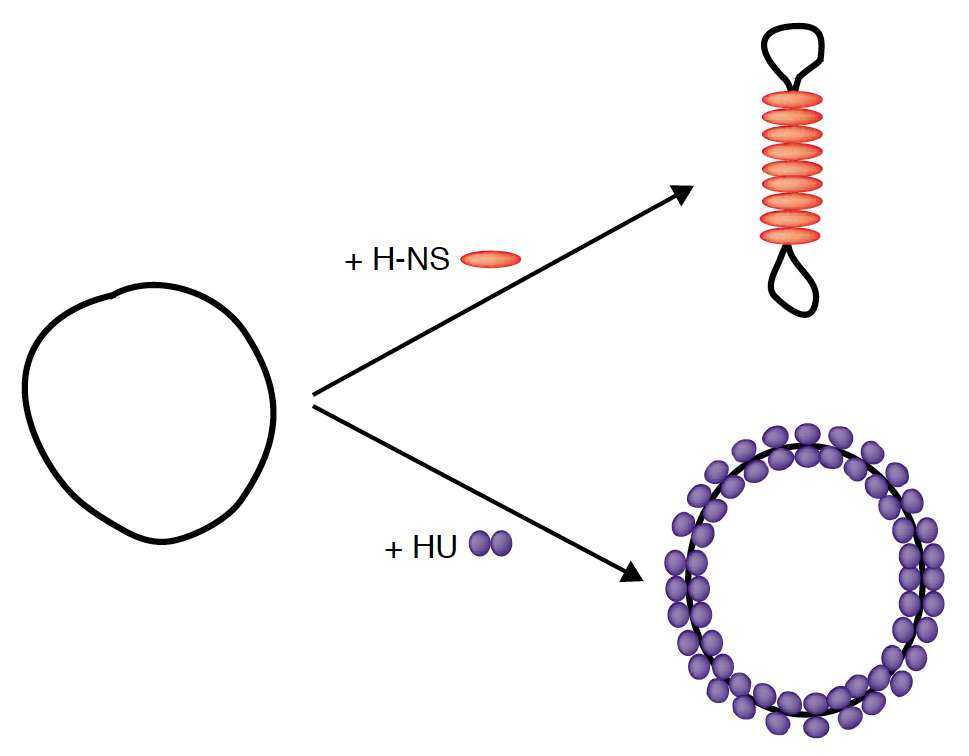
\includegraphics[width=8cm]{images/HUHNS.jpg}
    \caption{HU und H-NS sind Antagonisten.}
    \label{fig:huhns}
\end{figure}
\end{multicols}


\subsection{Factor for inversion stimulation (FIS)} \index{Nucleotid-associated Protein!Fis}
\begin{itemize}
    \item Induziert 50° bis 90° Biegungen
    \item es wird angenommen, dass es durch H-NS, IHF und CRP reguliert wird 
    \item 100 bis über 50'000 pro Zelle
\end{itemize}

\subsection{Integration Host Factor (IHF)} \index{Nucleotid-associated Protein!IHF}
\begin{itemize}
    \item induziert 160° bis 180° Biegungen
    \item verwandt mit Hu, aber nicht so konserviert
    \item Schlüsselrolle in CRISPR I und II Systemen  \index{CRISPR}
\end{itemize}


\subsection{DNA-binding protein from starved cells (Dps)} \index{Nucleotid-associated Protein!Dps}
\begin{itemize}
    \item Schutzprotein 
    \item Schützt vor oxidativen, stressbedingten Schäden
    \item Bindet Fe(II)
\end{itemize}

\subsection{MukBEF} \index{Nucleotid-associated Protein!MukBEF}
\begin{itemize}
    \item Condensin-ähnlich 
    \item Ringförmige Struktur
    \item Umkreist DNA und formt topologisch isolierte DNA Schleifen 
    \item unterstützt long-range interactions
    \item besteht aus mehreren Untereinheiten 
\end{itemize}
\begin{figure}[H]
    \centering
    \begin{subfigure}{0.25\textwidth}
    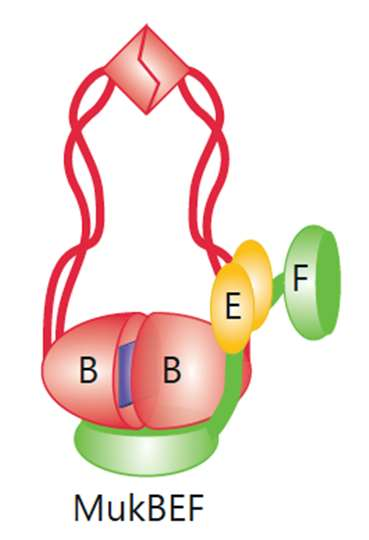
\includegraphics[width=\textwidth]{images/MUKBEF2.jpg}
    \caption{MukBEF}
    \label{fig:mukbefnorm}
\end{subfigure}
\hfill
\begin{subfigure}{0.4\textwidth}
    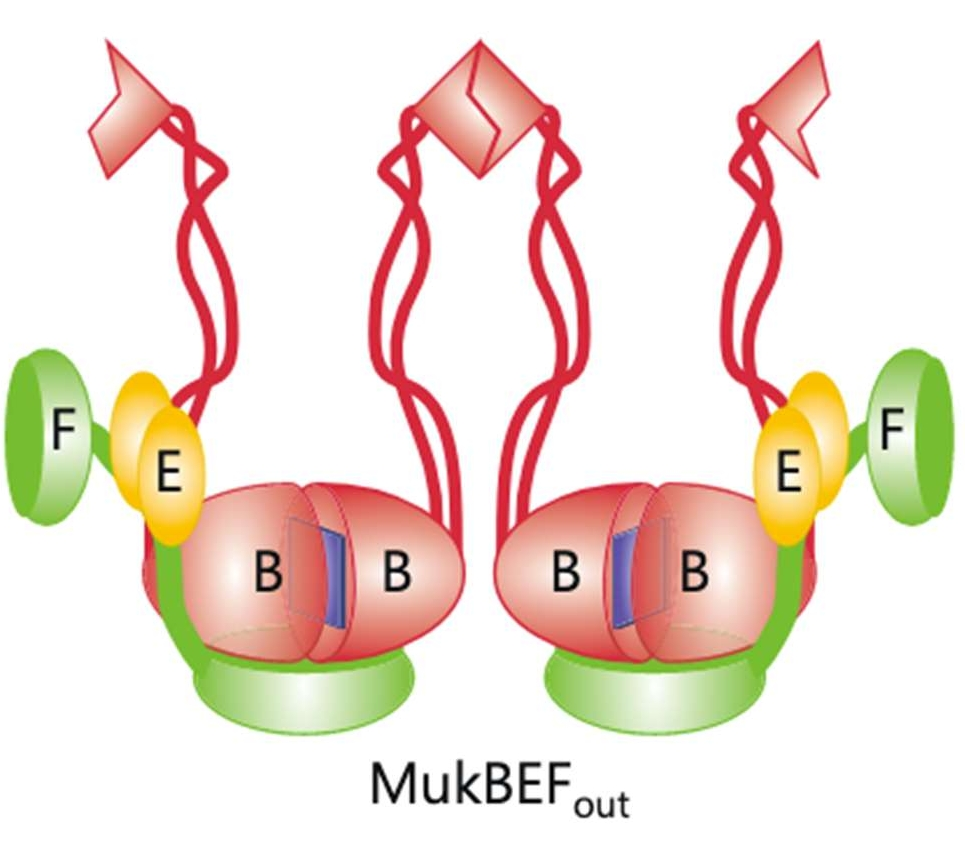
\includegraphics[width=\textwidth]{images/mukbefout.jpg}
    \caption{MukBEF out}
    \label{fig:mukbefout}
    \end{subfigure}
    \caption{Mögliche Organisationen von MukBEF.}
    \label{fig:mukbef}
\end{figure}

\subsection{\gls{smc}}
\begin{mybox}[title=Unterschied zwischen MukBEF und SMC]
MukBEF ist ein Proteinkomplex und SMC-Proteine sind eine Familie von Proteinen. MukBEF ist spezifisch für bestimmte Bakterien, wie z.B. Escherichia coli, während SMC-Proteine sind in vielen Organismen vorhanden sind.  \index{Nucleotid-associated Protein!MukBEF} \index{Nucleotid-associated Protein!SMC}
\end{mybox}
\section{Organsations des bakteriellen Genoms}
% Spatial arrangement (Folie 33) rausgelassen
Das bakterielle Genom besteht aus einem oder mehreren zirkulären oder linearen Chromosomen und oft noch weiteren \Glspl{plasmid}n. 
\begin{table}[H]
    \centering
    \begin{tabular}{p{1cm}p{3cm}p{3cm}p{3cm}p{3cm}}
        \textbf{Genom} & \textbf{Macrodomäne} & \textbf{\gls{cid}} & \textbf{\gls{hdr}} & \textbf{Microdomäne} \\ \\
        Helix & ausgeprägtes NAP-Bindungsprofil; hohe intra-Domänen-Rekombination & hohe Intra-Domänen Interaktionsfrequenz & hohe lokale DNA-Dichte & gegenseitig bedingte Genexpression; hohe intra-Domänen-Rekombination
    \end{tabular}
    \caption{Organsationsdomänen des bakteriellen Genoms.}
    \label{tab:Organsationsdomänen}
\end{table}
\noindent Nicht jeder Organimus besitzt jede Domäne! 
\begin{mechanism}[title=Wie viele Genome gibt es in einem typischen Prokaryoten?]
Ein Bakterium wäre ein typischer Prokaryot. Bakterien haben typischerweise ein Chromosom als Hauptgenom und das Plasmidgenom. 
\end{mechanism}

\section{Gentransfer} \index{DNA!Transfer}
\begin{table}[H]
    \begin{tabular}{p{4cm}p{11cm}}
        Konjugation \index{Konjugation} & Vorübergehende Verschmelzung von Einzellern zum Zwecke des sexuellen Austauschs von genetischem Material
Material  \\
       Transformation \index{Transformation}  & \textit{Vererbbare} Veränderung in einer Zelle oder einem Organismus, die durch exogene DNA hervorgerufen wird \\
       Transduktion \index{Transduktion} & Durch Viren vermittelter Gentransfer von einem Bakterium auf ein anderes
    \end{tabular}
    \caption{Mechanismen des prokaryotischen DNA-Transfers.}
    \label{tab:prokdnatransfer}
\end{table}

\subsection{Konjugation} 
\begin{figure}[H]
    \centering
    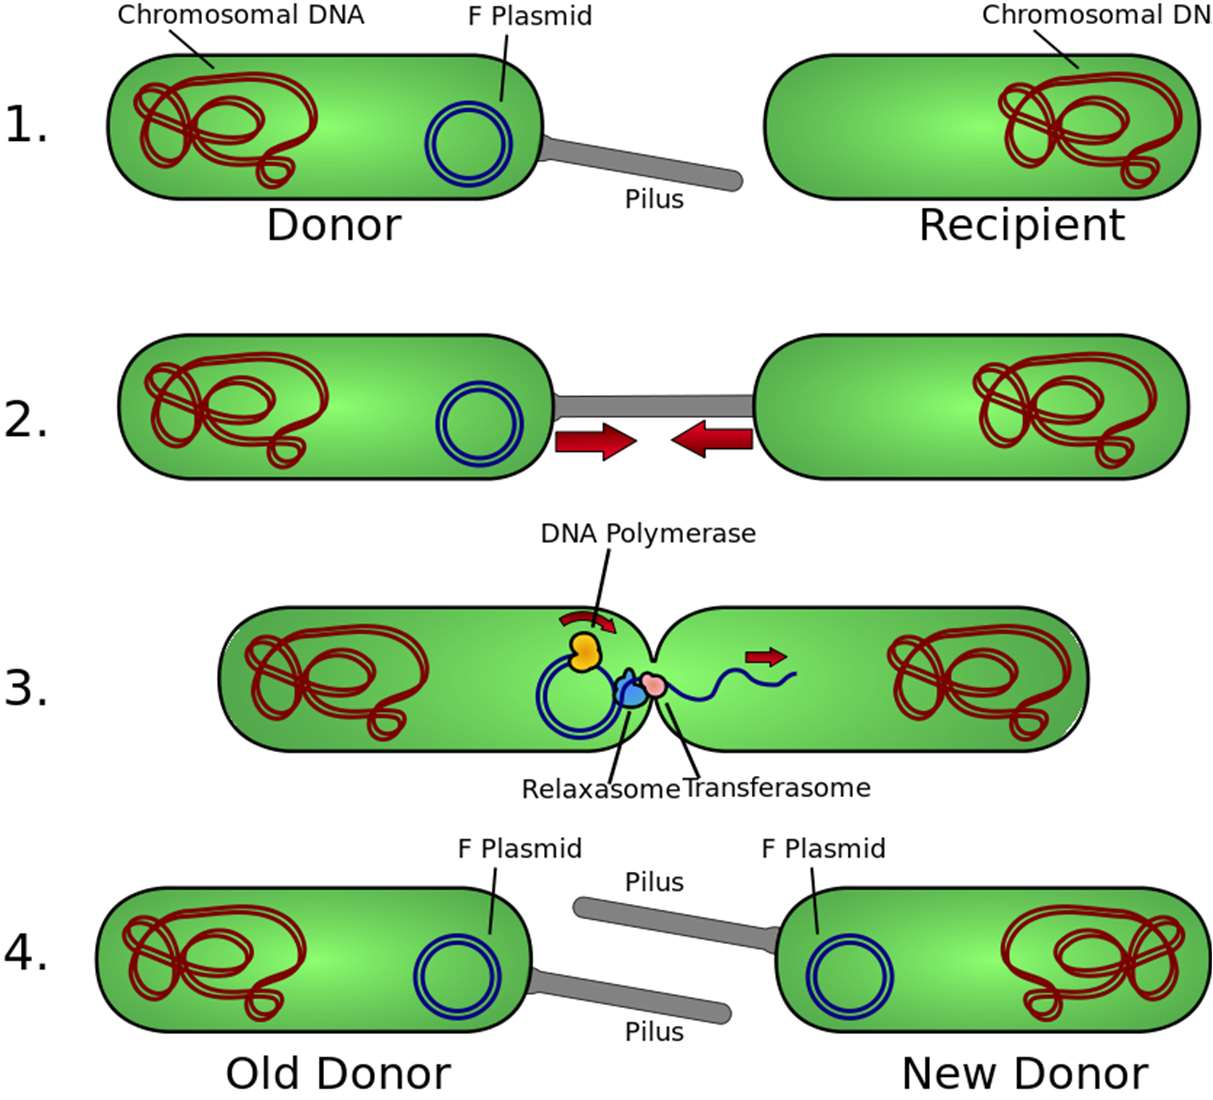
\includegraphics[width=10cm]{images/bakteriensex.jpg}
    \caption{Konjugation.}
    \label{fig:Konjugation}
\end{figure} \index{Konjugation} \index{Rezipient} \index{Donor}
\begin{mybox}[title=Horizontaler und vertikaler Gentransfer]
Vertikaler Gentransfer erfolgt von Eltern zu Nachkommen und ist ein grundlegender Mechanismus der Vererbung in der Evolution und horizontaler Gentransfer geschieht zwischen nicht verwandten Organismen und ermöglicht eine schnelle genetische Anpassung und Vielfalt.
\end{mybox} \index{Gentransfer} \index{Gentransfer!vertikaler}
\subsubsection*{F-Faktor} \index{F-Faktor}
 Verleiht Bakterien die Fähigkeit zur Konjugation \index{Konjugation} \index{F-Faktor} (horizontaler Gentransfer) \index{Gentransfer!horizontaler} und ermöglicht einen gerichteten Gentransfer vom Spender zum Empfänger. \index{Konjugation} \\
 Während der Konjugation wird die DNA des \gls{fplasmid}s repliziert, wobei eine neue Kopie in die in die Empfängerzelle und wandelt sie in F+ um.
\begin{multicols}{2}

\begin{figure}[H]
    \centering
    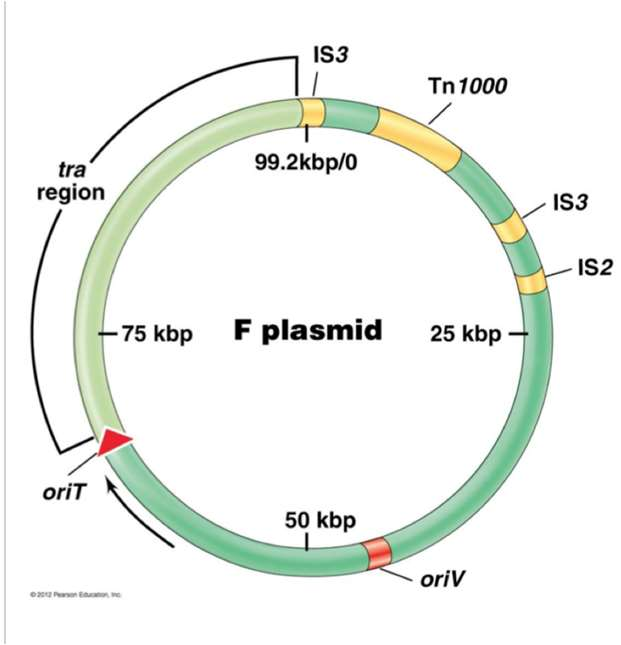
\includegraphics[width=6cm]{images/fplasmid.jpg}
    \caption{Aufbau des \gls{fplasmid}s.}
    \label{fig:fplsmid} 
\end{figure} \index{Plasmid!F-} \index{Plasmid!F-}
\columnbreak
\begin{table}[H] 
    \centering
    \begin{tabular}{p{2cm}p{4cm}}
       IS 3 / IS 2  &  insertion sequences \\
     oriV \index{oriV} & origin of replication \\
     oriT \index{oriT} & origin of conjugal transfer \\
     tra \index{tra} & transfer functions \index{oriV} \index{oriC} \index{tra}
    \end{tabular}
\end{table}
\end{multicols}
Die tra-Region des F-Faktors \index{F-Faktor} kodiert für ~35 Proteine, die in zwei Klassen unterteilt werden können: \index{Plasmid!F-} \index{F-Faktor} \\
\begin{enumerate}
\index{Protein!Mpf-}
    \item Mpf-Proteine (mating pair formation) 
    \begin{itemize}
    \item vermitteln den Zellkontakt und den DNA-Transport
        \item organisiert in Operons
        \item kodieren Proteine, die sich zu einer großen  makromolekulare Struktur, die als Typ-IV-Sekretionssystem bezeichnet wird
    \end{itemize}
    \index{Protein!Dtr-}
    \item Dtr-Proteine (DNA-Transfer und -Relaxation) 
    \begin{itemize}
    \item erfüllen Funktionen beim Einzelstrang-Nicking \index{Nicking!Einzelstrang} am oriT \index{oriT} und beim DNA-Transfer \index{DNA!Transfer} zum Exportsystem an der Membran
        \item kodieren Proteine, die sich an die DNA in der
der Ursprungsregion des Transfers, oriT, binden und eine Struktur namens Relaxosom bilden \index{Relaxosom}
    \end{itemize}
\end{enumerate}
\subsubsection{Nukleoproteintransport durch T4SS} \index{T4SS}
% Architecture of a conjugative T4SS rausgelassen (Folie 43 - 44)
\begin{enumerate}
    \item Schritt: Spenderzellen kommen mit Empfängerzellen in Kontakt. Der Zell-zu-Zell-Kontakt, der durch den Pilus \index{Pilus} vermittelt wird,
könnte durch spezifische Faktoren im Empfänger ausgelöst werden.
Empfänger ausgelöst werden. In diesem Stadium binden die Hilfsfaktoren
TrwA und IHF an die Origin of Transfer Region (oriT) \index{oriT} der plasmidischen DNA und die
Relaxase \index{Relaxase} schneidet sie an der nic-Stelle. 
\item Schritt : Bei Zellkontakt wird die Retraktion der
extrazellulären
Pilus \index{Pilus}
erleichtert
die
Interaktion zwischen den Membranen von
Spender- und Empfängerzellen, was zu einem
Membranfusionsprozess führt. Simulta-
oder vor dieser Membranfusion treibt das
Fusion treibt das Kopplungsprotein das
Relaxosom \index{Relaxosom}
in Richtung
die
Sekretion
kanal.
\item Schritt: Das Nukleoproteinsubstrat wird
auf VirB11 \index{VirB11} übertragen.
Die Relaxase \index{Relaxase} wird entfaltet und
wird durch den Kanal transloziert
kovalent an die DNA gebunden.
\item Schritt: VirB4 \index{VirB4} wird an der Basis des Sekretionskanals durch das Kopplungsprotein verdrängt, das die DNA-Translokation in Richtung 5'-3' unterstützt.
\end{enumerate}
\subsection{Transformation}
\begin{mybox}[title=Natüliche Kompetenz und induzierte Kompetenz]
Natürliche Kompetenz: Fähigkeit von Bakterien, DNA aus ihrer Umgebung aufzunehmen, ohne dass spezielle Behandlungen erforderlich sind. Diese Fähigkeit tritt unter natürlichen Bedingungen auf. \\ \index{Kompetenz!natürliche} \index{Kompetenz!induzierte}
Induzierte Kompetenz: Fähigkeit von Bakterien, DNA nach einer speziellen Behandlung (z.B. chemischen oder physikalischen Methoden) aufzunehmen. Diese Kompetenz wird künstlich hergestellt und ist häufig in Laboranwendungen zu finden.
\end{mybox}
\subsubsection{DNA-Uptake-Machinery} \index{DNA!Uptake-Machinery}
\begin{figure}[H]
    \centering
    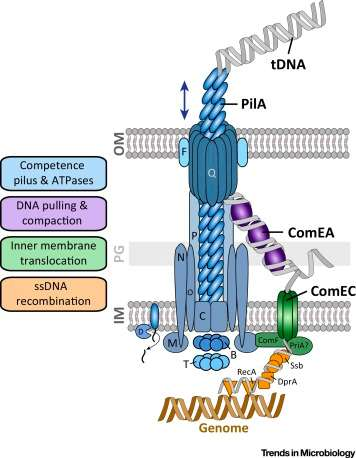
\includegraphics[width=8cm]{images/dnamachine.jpg}
    \caption{Modell der DNA-Aufnahmemaschinerie von natürlich kompetenten Vibrio cholerae. \\ (A) dsDNA is bound at the cell surface.  \\ (B) DNA is pulled through the type II secretin pore by retraction of a type 4 pilus (T4P).   \\ (C) One strand is translocated intact into the cytoplasm by the Rec2/ComEC protein; the other is degraded.  \\ (D) The new strand recombines with a homologous sequence in the chromosome, displacing the resident strand.}
    \label{fig:Aufnahmemaschinerie}
\end{figure} \index{Pilus}

\begin{figure}[H]
    \centering
    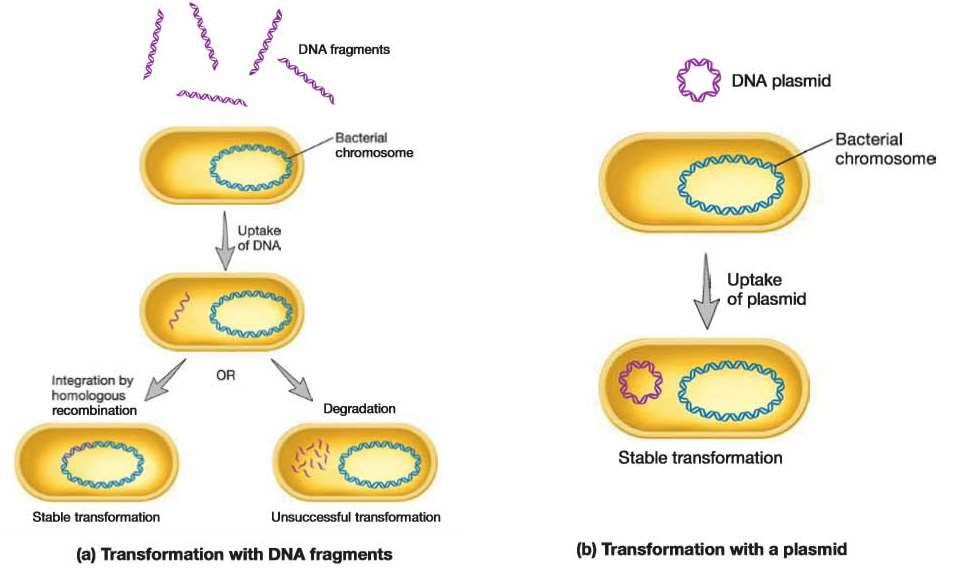
\includegraphics[width=12cm]{images/transformation.jpg}
    \caption{Transformationsabläufe.}
    \label{fig:transformation}
\end{figure}



\subsection{Transduktion}
\subsubsection{ = Gentransfer durch Viren}
\subsubsection{Entdeckung}
% TODO Mehr details
Die beiden Schenkel eines U-Rohres, die durch einen Filter getrennt sind, der nur für Partikel, die kleiner als die Bakterienzellen sind, durchlässig ist, werden mit zwei Stämmen von S. typhimurium \index{S. typhimurium} beschickt. \\
Nach einigen Stunden Inkubation konnte neben den Vertretern der beiden Stämme 1 und 2 Bakterien nachgewiesen werden, die sowohl Histidin als auch Tryptophan selbst herstellen konnten. Außerdem konnten freie Bakteriophagen (P22) in der Suspension, die zu Versuchsbeginn nicht vorhanden waren, beobachtet werden. \\
Da die Bakterien nicht direkt miteinander in Kontakt treten konnten, war eine Konjugation ausgeschlossen. Ebenfalls ausgeschlossen werden konnte eine Transformation, da keine freie DNA in den beiden Schenkeln des U-Rohres zu finden war. Als Schlussfolgerung ergab sich, dass die Bakteriophagen\index{Bakteriophage} Teile des Genoms von Bakterien des einen Stammes auf Zellen des anderen Stammes übertragen hatten. 
\begin{figure}[H]
    \centering
    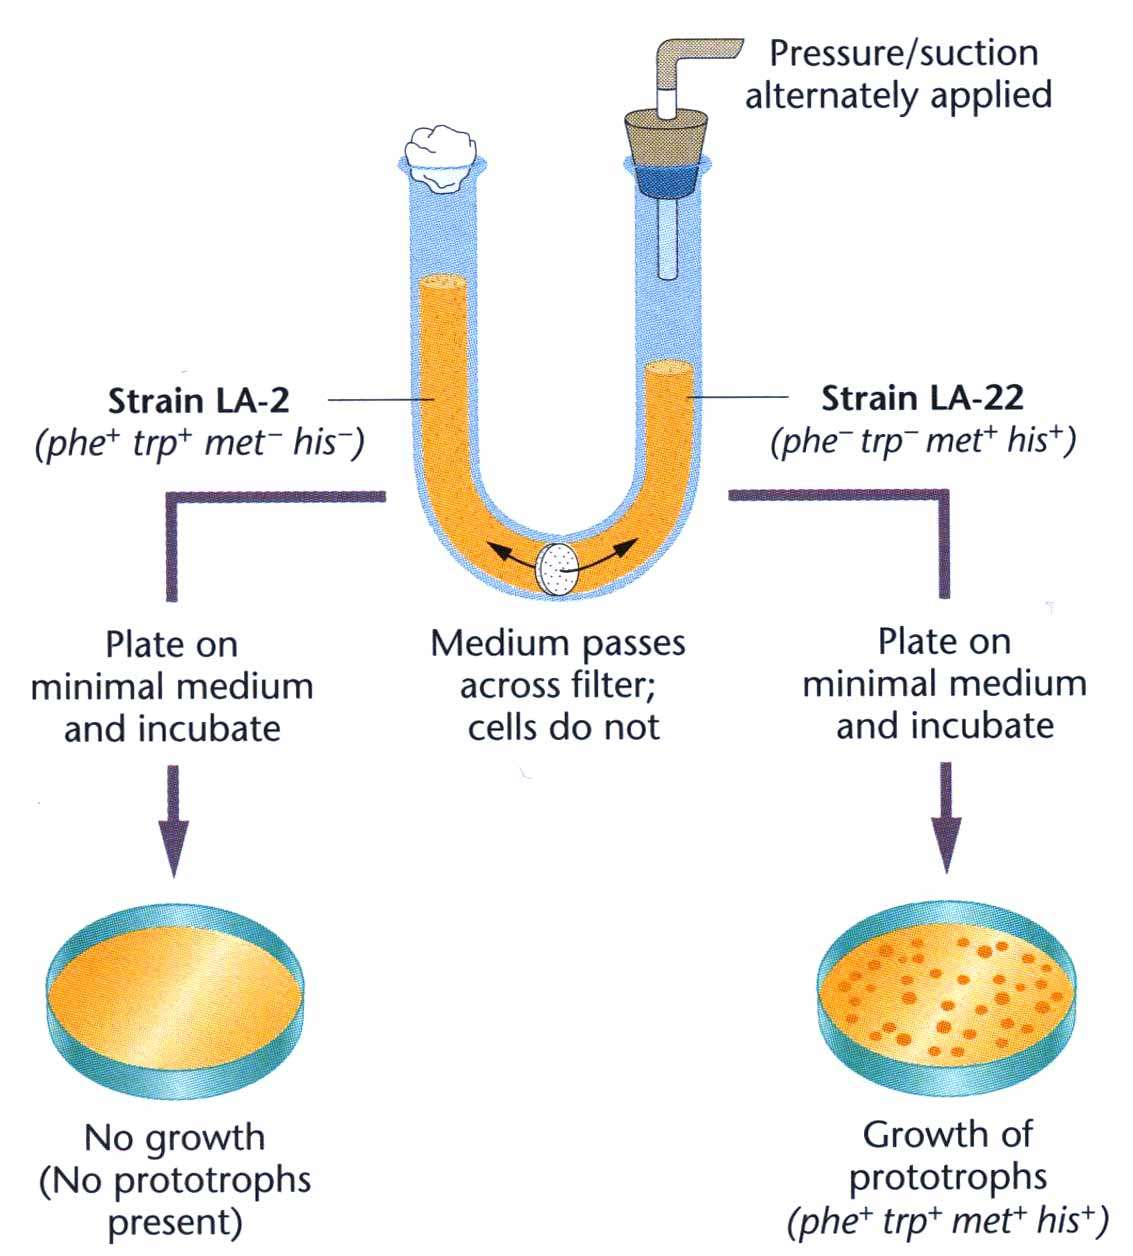
\includegraphics[width=8cm]{images/transductionentdeckung.jpg}
    \caption{Entdeckung der Transduktion.} 
    \label{fig:transductionentdeckung}
\end{figure} \index{Transduktion}

\subsubsection{Bakteriophagen}
\begin{multicols}{2}
\noindent Bakteriophagen \index{Bakteriophage} sind Viren, die bakterielle Zellen infizieren. Für ihre Vermehrung benötigen sie eine Bakterienzelle. Nach der Infektion der Bakterienzelle werden die Phagenkomponenten
synthetisiert und zusammengebaut.
\begin{figure}[H]
    \centering
    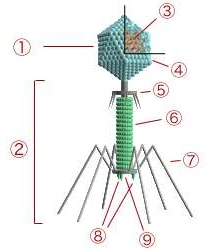
\includegraphics[width=5cm]{images/phagenaufbau.jpg}
    \caption{Aufbau von Bakteriophagen.} 
    \label{fig:phagenaufbau}
\end{figure} \index{Bakteriophage}
\noindent Montage der Phagen: 
\begin{enumerate}
    \item Montage des Kopfes und DNA-Verpackung
    \item Montage des Schwanzes
    \item Synthese und Montage der Schwanzfasern
\end{enumerate}
\columnbreak
\begin{figure}[H]
    \centering
    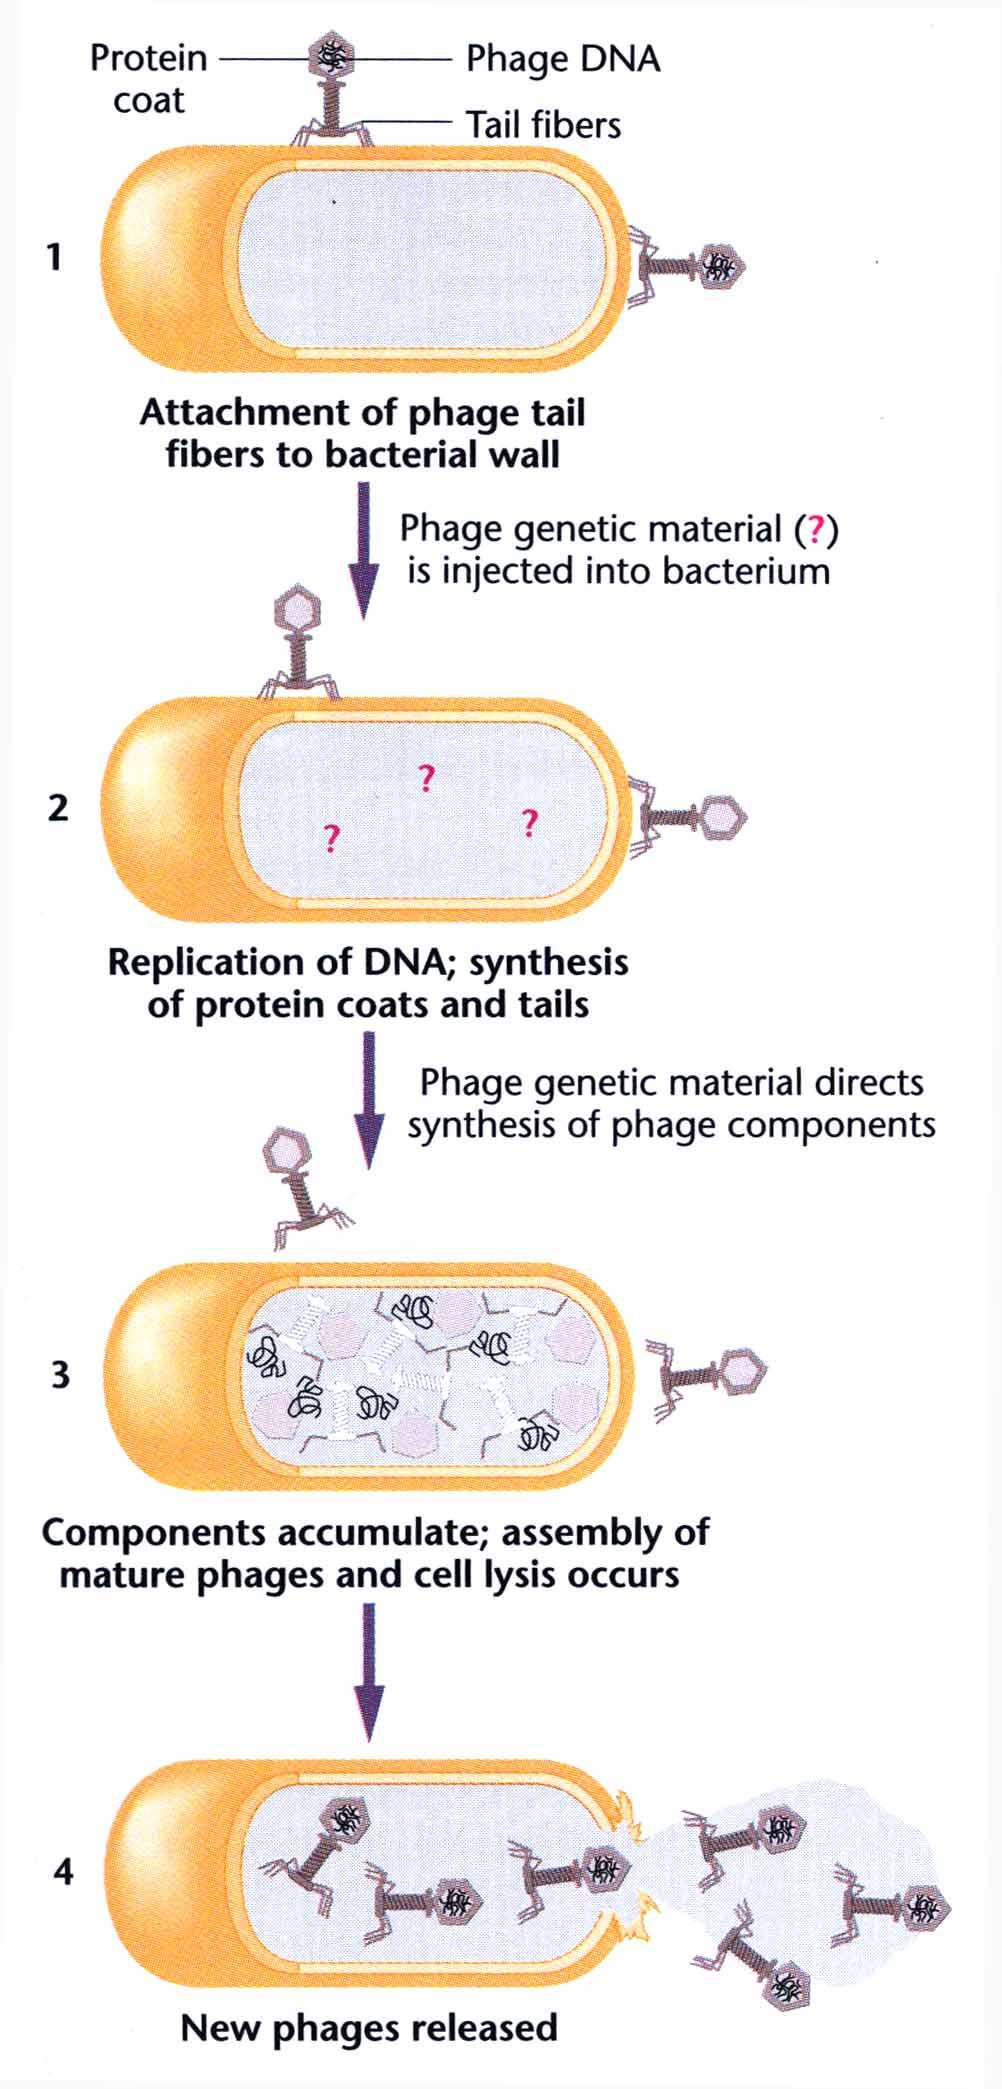
\includegraphics[width=5cm]{images/phagenfortpflanzung.jpg}
    \caption{Vermehrungszyklus von Bakteriophagen.} 
    \label{fig:phagenfortpflanzung}
\end{figure} \index{Bakteriophage}
\end{multicols}
\noindent DNA kann von einer Bakterienzelle auf eine andere übertragen werden
Zelle auf eine andere durch allgemeine Transduktion \index{Transduktion!allgemeine} übertragen werden. Die homologe Rekombination führt zum Austausch eines Abschnitts des Genoms. Die kotransduzierten Gene sind im Chromosom miteinander verbunden.
\begin{mybox}[title=Transduktion vs. generelle Transduktion]
Transduktion ist ein allgemeiner Begriff für den Prozess der Genübertragung durch Phagen, während die generelle Transduktion eine spezifische Form davon ist, die es Bakteriophagen ermöglicht, beliebige DNA-Stücke des Wirtsbakteriums zu übertragen. \index{Transduktion!generelle} \index{Transduktion} \index{Bakteriophage}
\end{mybox}


\section{Kartierung von prokaryotischen Genomen}
\index{Kartierung!Genom}
\subsection{Via Konjugation mit Hfr-Bakterien}
\index{Konjugation} \index{Hfr-Bakterien}
\subsubsection{Eigenschaften von hfr-Stämmen}
\begin{itemize}
    \item Hfr (high frequency of recombination)
    \item Entstehen durch Integration eines \gls{plasmid}s in das Chromosom
    \item Unterscheiden sich im Ort der Plasmidintegration \index{Plasmidintegration}
    \item werden bei der Chromosomenkartierung \index{Kartierung!Chromosomen} verwendet
\end{itemize}
Man kann m. H. von unterbrochener Konjugation Genkarten erstellen. \\
 Dabei werden verschiedene Hfr-Stämme als DNA-Donoren während der Konjugation von den DNA-Rezipienten\index{Rezipient} mittels mechanischer Scherkräfte in einem Standmixer (Waring blender) getrennt. Die Dauer der Konjugationen werden gemessen und man untersucht, welche Gene zu welcher Zeit transferiert wurden. Deswegen sind diese Genkarten in Minuten skaliert. \\
 Die Übertragung erfolgt an dem Ursprung, der durch den Ort der Integration des \gls{fplasmid}s in das Chromosom. Die Richtung der Übertragung wird durch die Ausrichtung des in das Chromosom integrierten \gls{fplasmid}s
\begin{mechanism}[title=Wodurch zeichnen sich bakterielle HFR-Stämme aus?]
\textbf{hfr}: DNA effizient von einem Bakterium in ein anderes übertragen (Übertragung vom \gls{fplasmid} und banachbarten Chromosomenregionen) \\
\textbf{Integriertes Plasmid}: \gls{fplasmid} (Fertility-Plasmid) ist in das Chromosom eines Bakteriums integriert 
\end{mechanism}
\begin{mechanism}[title=Wie entstehen bakterielle HFR-Stämme?]
Indem ein \gls{fplasmid} (Fertility-Plasmid) durch homologe Rekombination in das Chromosom eines Bakteriums integriert wird. 
\end{mechanism}
\begin{mechanism}[title=Worin unterscheiden sich unterschiedliche HFR-Stämme?]
In der Position der Integration des \gls{fplasmid}s und den Genen des integrierten \gls{fplasmid}s und somit den daraus resultierenden Eigenschaften.
\end{mechanism}
\begin{mechanism}[title=Wofür werden HFR-Stämme verwendet?]
In der Mikrobiologie und Genetik, um Gene zu kartieren und die Geninteraktionen innerhalb von Bakterien zu untersuchen
\end{mechanism}


 

\subsection{Via Transformation}
Man kann Transformation\index{Transformation} für die Genomkartierung\index{Kartierung!Genom} nutzen, indem man Plasmide als \glspl{vektor} nutzt und genomische DNA-Bibliotheken\index{DNA!Bibliothek} erstellt.  

\subsection{Restriktionsendonukleasen} \index{Restriktionsendonuklease} \label{sec:Restriktionsendonuklease}
\index{Endonuklease!Restriktions}
Restriktionsenzym sind Enzyme, die doppelsträngige DNA an bestimmten Stellen schneiden. Die Restriktion führt je nach Restriktionsenzym\index{Restriktionsenzym} zu klebrigen oder stumpfen DNA-Enden. Restriktionsenzyme können zum Klonen und zur Erstellung physikalischer DNA-Karten verwendet werden. \\ 
Siehe auch \nameref{sec:Restriktionskartierung} auf \pageref{sec:Restriktionskartierung}

\subsection{Klonierung} \index{Klonierung} \label{sec:klonierung}
\begin{figure}[H]
    \centering
    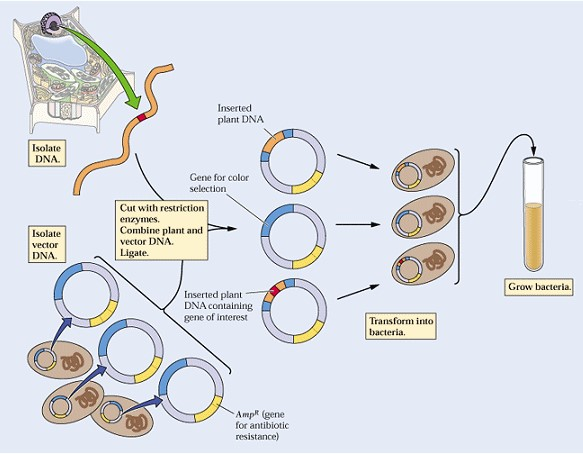
\includegraphics[width=10cm]{images/klonierung.jpg}
    \caption{Ablauf einer Klonierung.} 
    \label{fig:phagenfortpflanzung}
\end{figure}
\begin{mechanism}[title=Beschreiben sie die Isolierung von Plasmid-DNA]
\begin{itemize}
    \item DNA und \gls{vektor}-DNA isolieren \index{Vektor}
    \item DNAs mit Restriktionsenzymen\index{Restriktionsenzym} schneiden
    \item Isolierte DNA und \gls{vektor}-DNA kombinieren und ligieren
    \item Transformation\index{Transformation} in Bakterien 
    \item Bakterien kultivieren
\end{itemize} 
\end{mechanism}
\begin{mechanism}[title=Nennen Sie die drei wichtigsten Komponenten der Klonierung und ihre Funktion.]
\begin{itemize}
    \item \gls{vektor} – überträgt DNA
    \item \gls{sds}\index{SDS-Page} – Darstellung
    \item \gls{gfp} – Marker \index{GFP}
\end{itemize}
\end{mechanism}
\begin{mechanism}[title=Wofür steht SDS-Page? Was wird damit gemacht?]
\gls{sds} steht für Sodium Dodecylsulfat-Polyacrylamidgelelektrophorese und ist eine Methode um Proteine nach Masse zu trennen. Es wird bei der 2D Gelelektrophorese als zweite Dimension verwendet.
\end{mechanism}


\subsection{Restriktionskartierung} \index{Kartierung!Restriktions}
Zeigt die Positionen und Abstände von Restriktionsschnittstellen in einem DNA-Molekül. Diese Karte wird erstellt, indem die DNA mit spezifischen Restriktionsenzymen\index{Restriktionsenzym} geschnitten wird, die an bestimmten Sequenzen der DNA binden und diese schneiden. Die resultierenden Fragmente werden dann analysiert, um die Abstände zwischen den Schnittstellen zu bestimmen.
\begin{enumerate}
    \item Eine Population von klonierten DNA-Fragmenten
wird vorbereitet
\item DNA-Fragmente werden mit Restriktionsenzymen\index{Restriktionsenzym} geschnitten
\item Die Restriktionsfragmente werden aufgetrennt
durch Gelelektrophorese \index{Gelelektrophorese}
\end{enumerate}

\subsection{Physische \Gls{contig} Karte} \index{Contig}
Zeigt die physische Anordnung von zusammenhängenden DNA-Fragmenten (Contigs)in einem Genom. Sie wird erstellt, indem DNA-Fragmentsequenzen analysiert werden, um Überlappungen zu erkennen und eine durchgehende Sequenz darzustellen.


\section{Replikation von prokaryotischen Genomen} \index{Replikation}
\subsection{Unterschied zur eukaryotischen Replikation}
\begin{figure}[H]
    \centering
    \begin{subfigure}[t]{0.4\textwidth}
    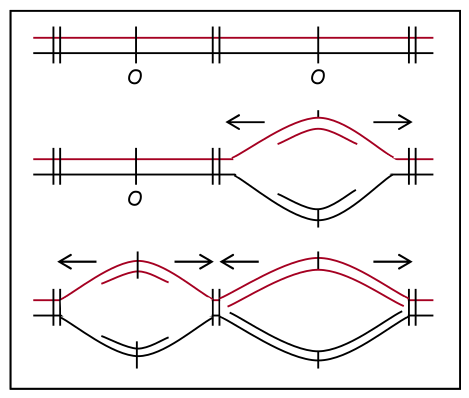
\includegraphics[width=\textwidth]{images/eukreplikation.png}
    \caption{Eukaryotische \glspl{replikon} sind klein und replizieren langsamer als prokaryotische \glspl{replikon}.}
    \label{fig:eukreplikation}
\end{subfigure} \index{Replikon}
\hfill
\begin{subfigure}[t]{0.4\textwidth}
    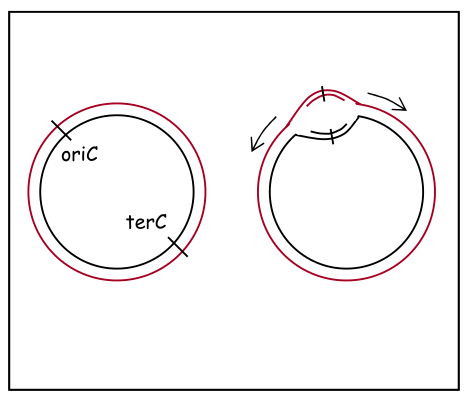
\includegraphics[width=\textwidth]{images/prokreplikation.png}
    \caption{Prokaryotische Chromosomen bestehen nur aus einem \gls{replikon}.}
    \label{fig:prokreplikation}
    \end{subfigure}
    \caption{Unterschied zwischen der eukaryotischen Replikation und der prokaryotischen Replikation.}
    \label{fig:replikationen}
\end{figure}
\begin{mechanism}[title=Definition Replikon]
DNA- oder RNA-Abschnitt, der ausgehend von einem Replikationsursprung an einem Stück repliziert wird.
\end{mechanism}
\subsection{Bakterielle Replikationsursprünge} \index{Replikationsursprung}
Der \gls{oric} ist der Replikationsursprung im bakteriellen Chromosom und der \gls{oriv} ist der Replikationsursprung im \gls{plasmid}. 
\subsection{Replikation von linearen prokaryotischen Chromosomen} \index{Replikation}
\begin{figure}[H]
    \centering
    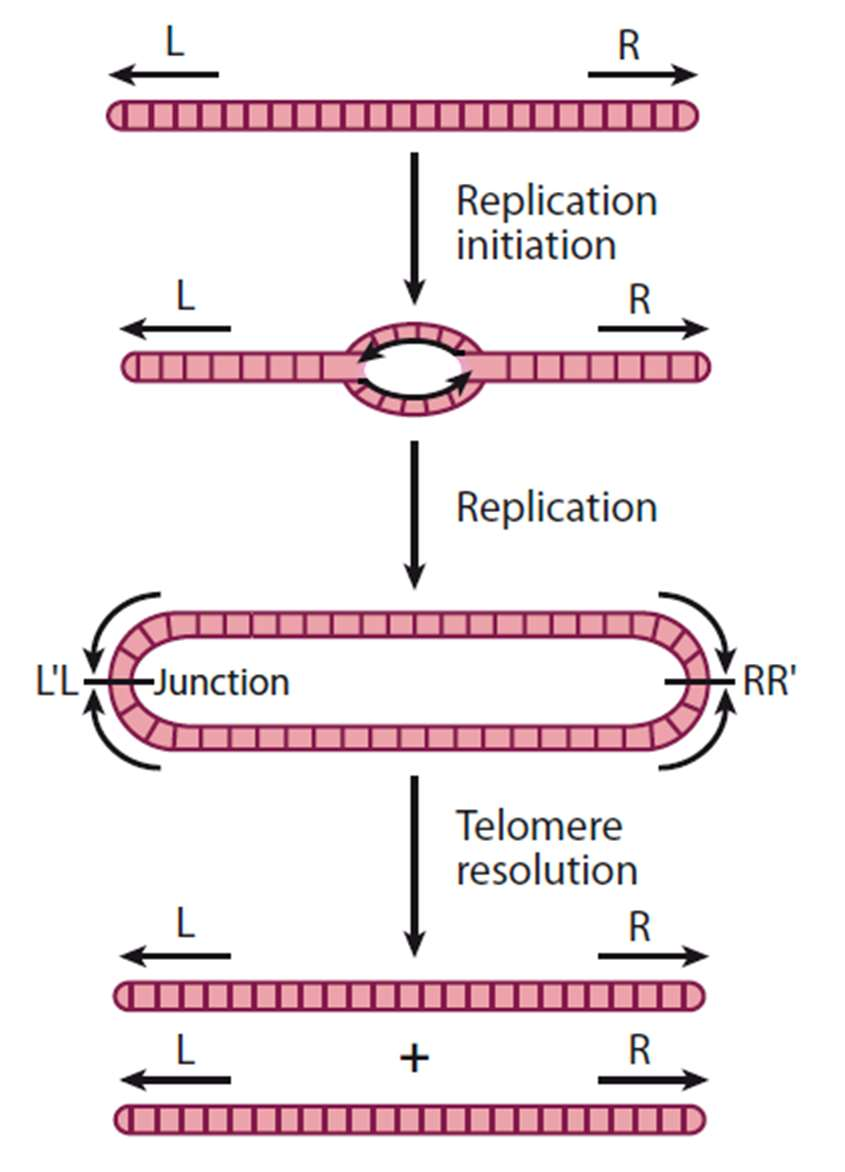
\includegraphics[height=8cm]{images/linear1.jpg}
    \caption{Normale lineare Replikation mit \glspl{telomer}n.}
    \label{fig:linearrepl}
\end{figure} \index{Telomer}
\begin{figure}[H]
    \centering
    \begin{subfigure}[t]{0.4\textwidth}
    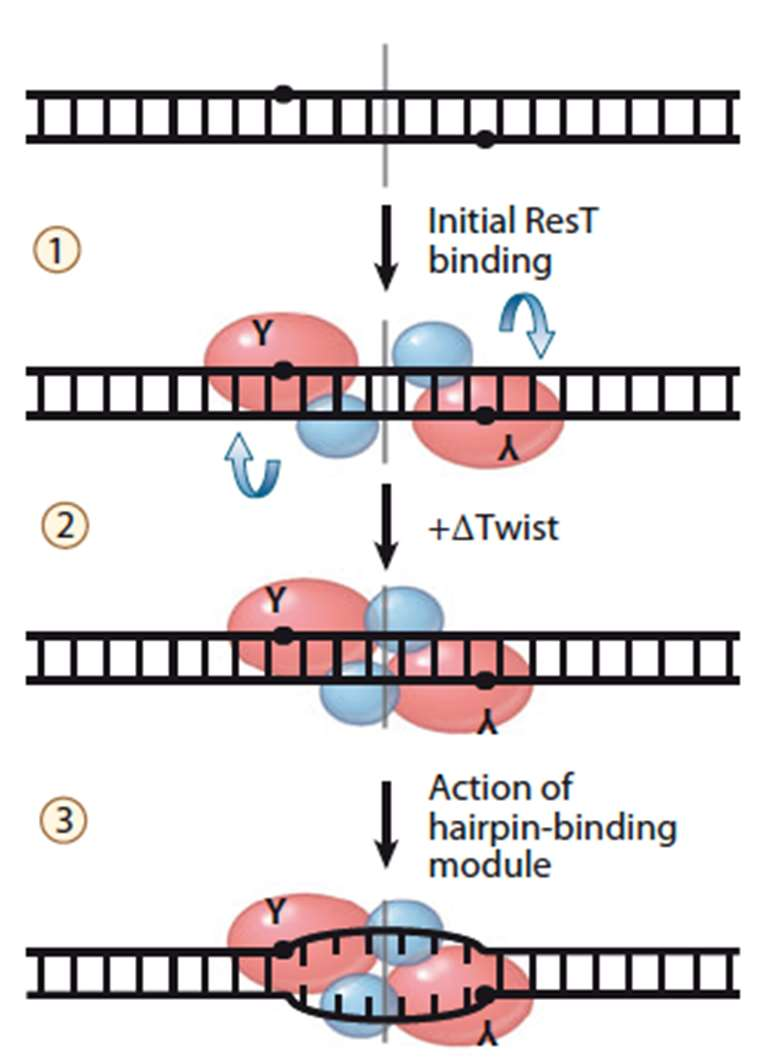
\includegraphics[width=\textwidth]{images/linear2.jpg}
\end{subfigure}
\hfill
\begin{subfigure}[t]{0.4\textwidth}
    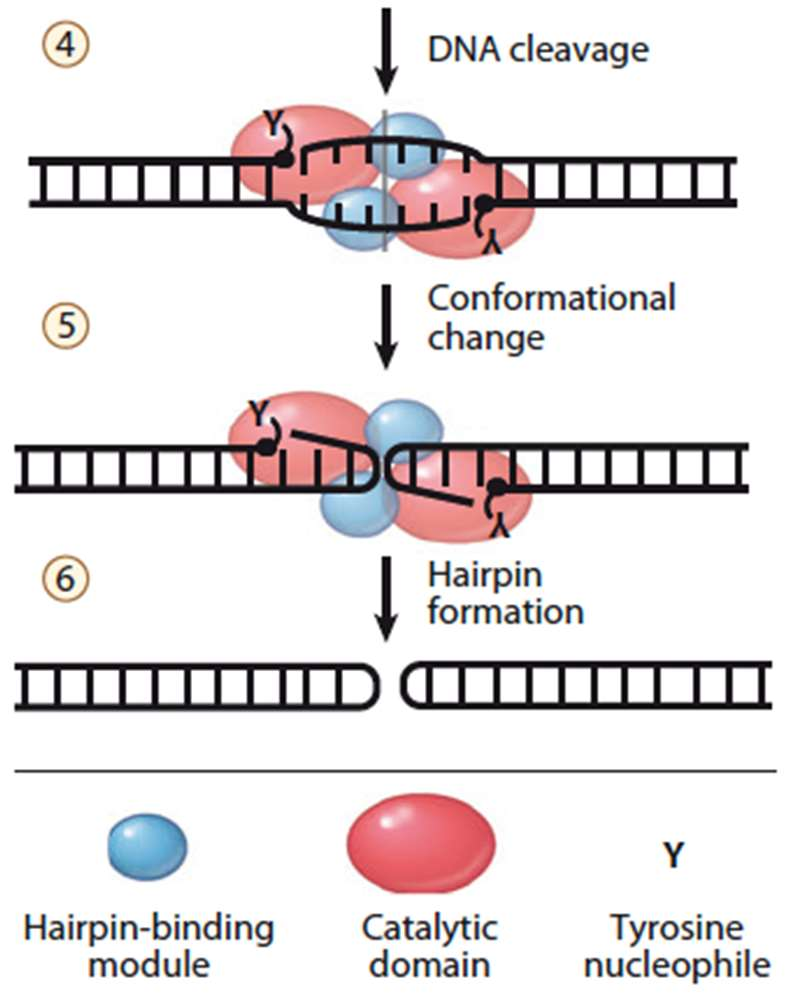
\includegraphics[width=\textwidth]{images/linear3.jpg}
    \end{subfigure} 
    \caption{Lineare Replikation unter Bildung von \glspl{haarnadelstruktur}} \index{Haarnadelstruktur}
    \label{fig:linearreplhairpin}
\end{figure}
\section{Der vegetative bakterielle Zellzyklus}
\begin{figure}[H]
    \centering
    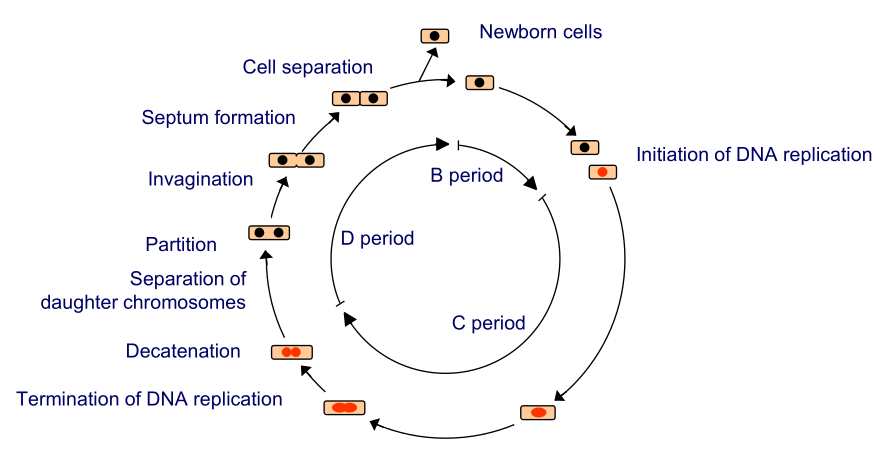
\includegraphics[width=15cm]{images/vegcellcycle.png}
    \caption{Der vegetative bakterielle Lebenszyklus.}
    \label{fig:vegcellcycle}
\end{figure}
\begin{figure}[H]
    \centering
    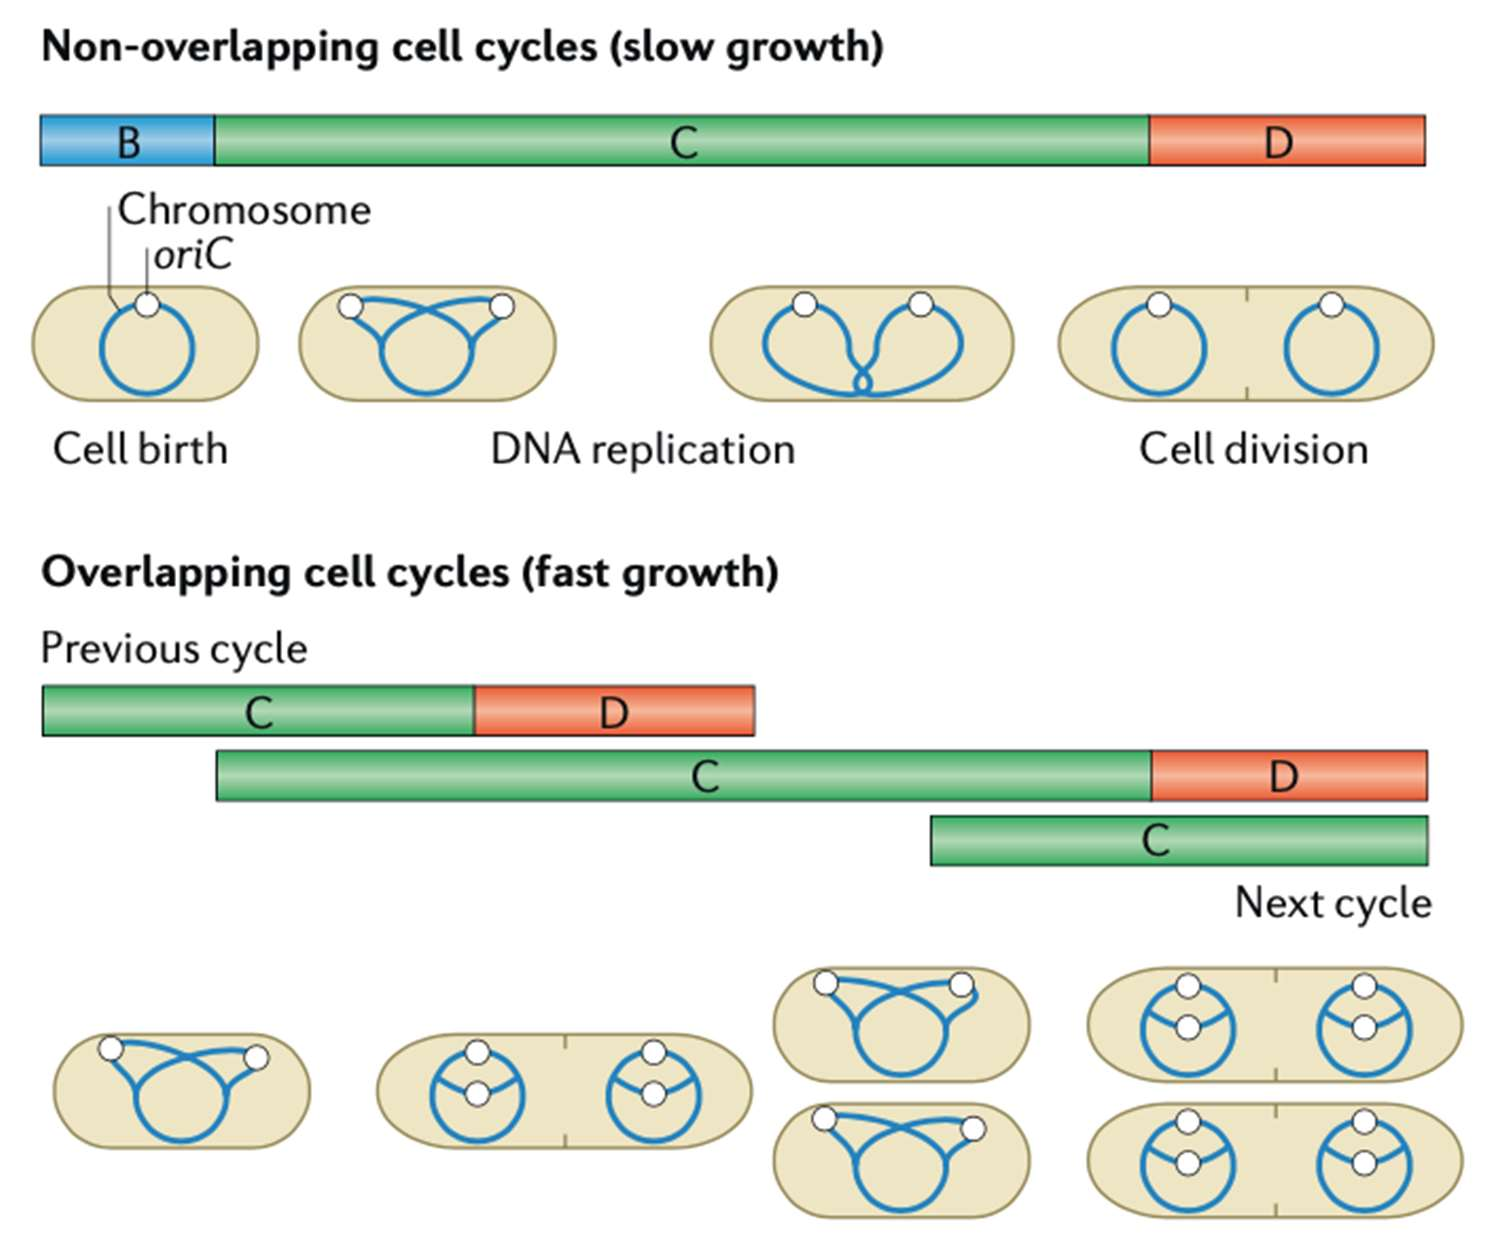
\includegraphics[width=12cm]{images/cellcycles.jpg}
    \caption{Sich überschneidende und nicht überschneidende Zellzyklen.}
    \label{fig:vegcellcycle}
\end{figure} \index{Zellzyklus}
